\chapter{Proof for rank 4}
\label{proof-4}

\paragraph{}
We study the different cases for polytopes of rank 4. By Lemma~\ref{min-4-trans}, we can have two, three or four 4-transposition.

\section{Preliminary results}

\begin{theorem}
  Neither $\rho_1$ nor $\rho_2$ can be a 2-transposition.
\end{theorem}

\begin{proof}
  Suppose that $\rho_1$ is a 2-transposition. They must be at least two 4-transpositions out of the three other involutions. Thus $\rho_0$ or $\rho_3$ must be a 4-transposition.

  \paragraph{}
  \textbf{$\rho_0$ is a 4-transposition}

  \paragraph{}
  If the $\rho_0$ edge are not part of any alternating square, by Lemma~\ref{rho0AtEnd}, they needs one $\rho_1$ edge each to be connected to the graph. But that is impossible because there are only two $\rho_1$ edge for four $\rho_0$ edges. Thus the $\rho_0$ edges must be part of an alternating square and moreover no $\rho_1$ edges can be part of an alternating square except if all $\rho_0$ edges are part of an alternating square.

  \paragraph{}
  There are multiple possibilities for the square: $[\rho_0, \rho_1]$, $[\rho_0, \rho_2]$ and $[\rho_0, \rho_3]$. The first possibility contains a $\rho_1$ edge and thus is impossible. If the alternating square is $[\rho_0, \rho_3]$, it must still be part of a sequence of alternating square. And the adjacent alternating square can be $[\rho_0, \rho_2]$ or $[\rho_1, \rho_3]$. The last case is not possible because it contains a $\rho_1$ edge.

  \paragraph{}
  Thus an alternating square must be $[\rho_0, \rho_2]$, this alternating square can be extended into a sequence. The possible adjacent alternating squares are $[\rho_1, \rho_2], [\rho_0, \rho_1]$ and $[\rho_0, \rho_3]$. The sequence cannot be extended twice in the same direction, and if it is extended once on both side, it cannot be connected to anything. Thus no $\rho_1$ edges can be part of an alternating square. The only possibility is the last one: $[\rho_0, \rho_3]$.

  \paragraph{}
  If the sequence is not extended.\footnote{Continue}

  \paragraph{}
  \textbf{$\rho_3$ is a 4-transposition}

  \paragraph{}
  If $\rho_3$ is a 4-transposition, only one alternating square can be built with $\rho_1$. Thus the two other must used single or double edge. By simplicity we consider simple edge for now. The edges can be doubled later. Two $\rho_2$ edges are needed in order to link this. But all $\rho_1, \rho_2$

\end{proof}

\paragraph{}
We start by proving some lemmas that are used when there are used for the cases with three or four 4-transpositions. We suppose in the following proofs that if there is a 2-transition, then it is $\rho_0$. This can be done with the previous theorem and by using the duality.

\begin{lemma}
  Let $\Gamma$ be a sggi of rank 4 on $A_{11}$ in which $\rho_1, \rho_2$ and $\rho_3$ are 4-transpositions, in the permutation representation graph of $\Gamma_{\rho_1, \rho_3}$, there must be a least one single $\rho_1$ edge (and thus a single $\rho_3$ edge).
\end{lemma}

\begin{proof}
  By Lemma~\ref{adjacent-must-not-commute}, a $\rho_0$ must be adjacent to a $\rho_1$ edge. The $\rho_1$ can be a single edge, a double edge with another involution or on an alternating square in $\Gamma_{\rho_1, \rho_3}$.

  \paragraph{}
  If the $\rho_1$ edge is part of a double edge $(\rho_1, \rho_3)$. But if the $\rho_0$ and $\rho_1$ do not commute then $\rho_0$ does not commute with $\rho_3$ and this is a contradiction with Proposition~\ref{intersection-patterns}.

  \paragraph{}
  If $\rho_1$ is on an alternating square $[\rho_1, \rho_3]$, the same occurs.

\end{proof}

\begin{lemma}
    If $\Gamma$ is a sggi of rank 4 on $A_{11}$ in which $\rho_1, \rho_2$ and $\rho_3$ are 4-transpositions, there cannot be more than one $\rho_1$ single edge and thus there cannot be more than one $\rho_3$ single edge in the graph of $\Gamma_{\rho_1, \rho_3}$.
\end{lemma}

\begin{proof}
  There are not enough points otherwise. Hence if they are two single $\rho_1$ edges, there are two single $\rho_3$ edges. Those 4 edges uses 8 points. The four last edges can be arranged in an alternating square or two double edges. Those edges uses 4 vertices. That is not possible because there are only 11 points.
\end{proof}

\begin{corollary}
  \label{rank-4-single-1}
    If $\Gamma$ is a sggi of rank 4 on $A_{11}$ in which $\rho_1, \rho_2$ and $\rho_3$ are 4-transpositions, there are exactly one $\rho_1$ single edge and one $\rho_3$ single edge in the graph of $\Gamma_{\rho_1, \rho_3}$.
\end{corollary}

\begin{lemma}
  \label{rank-4-3-patterns}
  Let $\Gamma$ be a sggi of rank 4 that generate $A_{11}$. If $\rho_1$, $\rho_2$ and $\rho_3$ are 4-transpositions then the patterns formed by $\rho_1$ and $\rho_3$ edges are one alternating square, one double edge and two simple edges (one for each involution).
\end{lemma}

\begin{proof}
  By Corollary~\ref{rank-4-single-1} there is exactly one $\rho_1$ single edge. The remaining possibilities for the three remaining edges of $\rho_1$ are limited: one alternating square $[\rho_1, \rho_3]$ and one double edge $(\rho_1, \rho_3)$ or three double edges $(\rho_1, \rho_3)$.

  \paragraph{}
  Suppose that there are three double edges. A $\rho_0$ edge must be placed next to the $\rho_1$ single edge.

    \begin{figure}[H]
      \begin{center}
        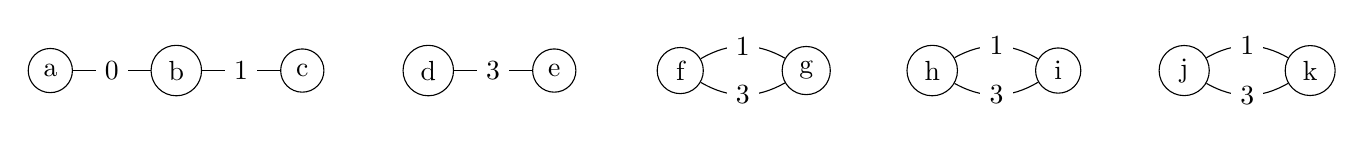
\begin{tikzpicture}[scale=.8]

          \begin{scope}[every node/.style={circle,draw}]
            \node (1)  at (0,0)   {a};
            \node (2)  at (2,0)   {b};
            \node (3)  at (4,0)   {c};
            \node (4)  at (6,0)   {d};
            \node (5)  at (8,0)   {e};
            \node (6)  at (10,0)  {f};
            \node (7)  at (12,0)  {g};
            \node (8)  at (14,0)  {h};
            \node (9)  at (16,0)  {i};
            \node (10) at (18,0)  {j};
            \node (11) at (20,0)  {k};
          \end{scope}

          \begin{scope}[every node/.style={fill=white}]

            \begin{scope}[every edge/.style={draw}]
              \path (1)  edge node {$0$} (2);
              \path (2)  edge node {$1$} (3);
              \path (6)  edge[bend left=30] node {$1$} (7);
              \path (8)  edge[bend left=30] node {$1$} (9);
              \path (10) edge[bend left=30] node {$1$} (11);
              \path (4)  edge node {$3$} (5);
              \path (6)  edge[bend right=30] node {$3$} (7);
              \path (8)  edge[bend right=30] node {$3$} (9);
              \path (10) edge[bend right=30] node {$3$} (11);
            \end{scope}
          \end{scope}

        \end{tikzpicture}
        \caption{}
      \end{center}
    \end{figure}

  \paragraph{}
  Now no $\rho_0$ edge can be connected to any point without being in an alternating square but there are three $\rho_0$ edges remaining, thus there must be two adjacent squares but that is impossible because there is not two chain of length at least 3. 
\end{proof}
